% =====================================================================
%  fig_bio_intracellular_map — Biological reading of the two-type model
%
%  Companion to Table 1 of sections/07_biological_application.tex.
%  Maps (X_t, Y_t, lambda_i, mu_i, nu, delta_i, tau_c) onto a single
%  macrophage-associated intracellular compartment.
%
%  Vector schematic.  Build:  bash build.sh   (-> ../fig_bio_intracellular_map.pdf)
%  Notation follows sections/02_model.tex and Table 1 exactly.
%
%  Deliberately NON-committal: equal arrow weights for delta_1 and
%  delta_2 (no regime privileged), schematic surface cue only, and the
%  extracellular aftermath is drawn as out-of-model.
% =====================================================================
\documentclass[tikz,border=6pt,11pt]{standalone}

\usepackage[T1]{fontenc}
\usepackage{lmodern}          % match the paper's Latin Modern text/math
\usepackage{amsmath,amssymb,mathtools}
\usepackage{xcolor}

\usetikzlibrary{arrows.meta,positioning,calc,backgrounds,fit,decorations.pathmorphing}

% ---- palette -------------------------------------------------------
% Canonical manuscript accents (Okabe--Ito; used for rate symbols,
% event arrows and type identity) -- identical to fig01/fig05.
\definecolor{type1}{HTML}{0072B2}
\definecolor{type2}{HTML}{D55E00}
\definecolor{cata}{HTML}{9A2820}
\definecolor{ink}{HTML}{1A1C1F}
\definecolor{inksoft}{HTML}{565B62}
\definecolor{rule}{HTML}{E3E6EA}

% Muted body tints for the drawn bacteria (same hue families, lowered
% chroma; type 1 deliberately lighter than type 2 so the two separate
% in greyscale as well as in hue).
\definecolor{t1body}{HTML}{7BA6C6}
\definecolor{t1edge}{HTML}{2E6A92}
\definecolor{t2body}{HTML}{A85A32}
\definecolor{t2edge}{HTML}{74381A}
\definecolor{t12body}{HTML}{9A8069}   % midpoint tint, conversion band

% Cell / compartment neutrals
\definecolor{cyto}{HTML}{F2F0EC}
\definecolor{cytoline}{HTML}{A9A29A}
\definecolor{nucleus}{HTML}{E7E3DC}
\definecolor{nucline}{HTML}{D2CCC3}
\definecolor{vac1}{HTML}{F7FAFC}
\definecolor{vac2}{HTML}{FDF7F2}
\definecolor{vacline}{HTML}{93A1AB}
\definecolor{outside}{HTML}{F6F6F5}
\definecolor{outsideline}{HTML}{C9C9C6}
\definecolor{catafill}{HTML}{F9EFEE}
\definecolor{keyfill}{HTML}{FBFAF8}

% =====================================================================
%  Bacterium glyphs (short rounded rods, drawn as round-capped strokes)
% =====================================================================
% #1 x, #2 y, #3 rotation
\newcommand{\rodOne}[3]{%
  \begin{scope}[shift={(#1,#2)},rotate=#3]
    \draw[line width=0.40cm,line cap=round,t1edge] (-0.23,0) -- (0.23,0);
    \draw[line width=0.32cm,line cap=round,t1body] (-0.23,0) -- (0.23,0);
  \end{scope}}

% type 2: faint halo + sparse schematic surface structures
\newcommand{\rodTwo}[3]{%
  \begin{scope}[shift={(#1,#2)},rotate=#3]
    \draw[line width=0.60cm,line cap=round,t2body,opacity=0.22] (-0.23,0) -- (0.23,0);
    \draw[line width=0.40cm,line cap=round,t2edge] (-0.23,0) -- (0.23,0);
    \draw[line width=0.32cm,line cap=round,t2body] (-0.23,0) -- (0.23,0);
    \foreach \s in {-0.17,-0.02,0.13}{%
      \draw[t2edge,line width=0.3pt] (\s,0.155) -- ++(0.025,0.135);
      \draw[t2edge,line width=0.3pt] (\s+0.05,-0.155) -- ++(0.025,-0.135);}
  \end{scope}}

% conversion-band rods: smaller, interpolated tint
\newcommand{\rodMid}[4]{%  x, y, rotation, body colour
  \begin{scope}[shift={(#1,#2)},rotate=#3]
    \draw[line width=0.31cm,line cap=round,#4!62!black] (-0.17,0) -- (0.17,0);
    \draw[line width=0.24cm,line cap=round,#4] (-0.17,0) -- (0.17,0);
  \end{scope}}

% released bacteria, out of model: pale, reduced opacity
\newcommand{\rodOut}[3]{%
  \begin{scope}[shift={(#1,#2)},rotate=#3,opacity=0.42]
    \draw[line width=0.38cm,line cap=round,inksoft] (-0.21,0) -- (0.21,0);
    \draw[line width=0.30cm,line cap=round,black!22] (-0.21,0) -- (0.21,0);
  \end{scope}}

% =====================================================================
%  Event glyphs: replication self-loop and loss-to-nothing
% =====================================================================
% #1 x, #2 y, #3 colour, #4 rate symbol, #5 word
\newcommand{\birthGlyph}[5]{%
  \begin{scope}[shift={(#1,#2)}]
    \draw[#3,line width=0.85pt,-{Stealth[length=1.5mm,width=1.3mm]}]
      (0.22,0.06) arc (-42:250:0.225);
    \node[#3,anchor=west,inner sep=0pt,font=\small] at (0.44,0.02) {#4};
    \node[inksoft,anchor=north,inner sep=0pt,font=\scriptsize] at (0.30,-0.30) {#5};
  \end{scope}}

\newcommand{\deathGlyph}[5]{%
  \begin{scope}[shift={(#1,#2)}]
    \draw[#3,line width=0.85pt,-{Stealth[length=1.5mm,width=1.3mm]}]
      (-0.30,0.02) -- (0.06,0.02);
    \node[inksoft,anchor=west,inner sep=0.5pt,font=\small] at (0.10,0.02) {$\varnothing$};
    \node[#3,anchor=west,inner sep=0pt,font=\small] at (0.44,0.02) {#4};
    \node[inksoft,anchor=north,inner sep=0pt,font=\scriptsize] at (0.20,-0.30) {#5};
  \end{scope}}

\begin{document}
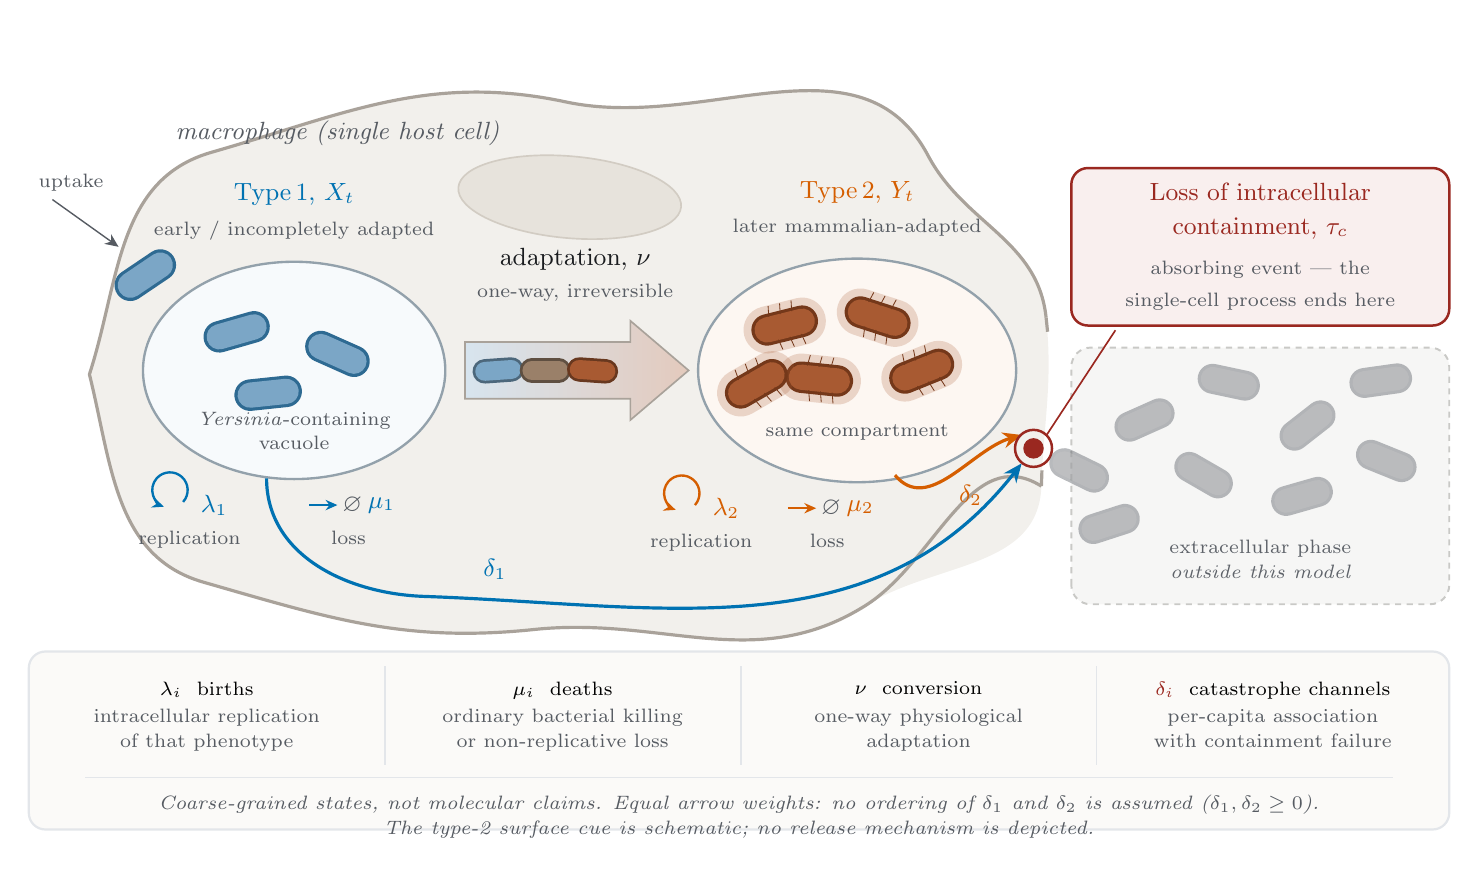
\begin{tikzpicture}[
    >={Stealth[length=2.4mm,width=2.0mm]},
    font=\normalsize,
    hazard/.style={line width=1.15pt,-{Stealth[length=2.4mm,width=2.0mm]}},
    lead/.style={inksoft,line width=0.5pt},
  ]

% =====================================================================
%  0.  Out-of-model extracellular panel (drawn first, sits behind)
% =====================================================================
\fill[outside,rounded corners=7pt] (12.62,-3.12) rectangle (17.42,0.14);
\draw[outsideline,line width=0.7pt,dash pattern=on 2.2pt off 2.0pt,rounded corners=7pt]
      (12.62,-3.12) rectangle (17.42,0.14);

\rodOut{13.55}{-0.78}{24}
\rodOut{14.62}{-0.30}{-12}
\rodOut{15.62}{-0.85}{38}
\rodOut{16.55}{-0.28}{8}
\rodOut{14.30}{-1.48}{-30}
\rodOut{15.55}{-1.75}{16}
\rodOut{16.62}{-1.30}{-22}

\node[inksoft,align=center,font=\scriptsize,opacity=0.95] at (15.02,-2.55)
     {extracellular phase\\[1pt]\itshape outside this model};

% =====================================================================
%  1.  Macrophage: fill, then stroked outline with a break at the right
% =====================================================================
\begin{scope}[on background layer]
\fill[cyto]
   (0.15,-0.20)
     to[out=72,in=196]   (1.70,2.62)
     to[out=16,in=168]   (6.20,3.26)
     to[out=-12,in=118]  (10.80,2.58)
     to[out=-62,in=96]   (12.30,0.52)
     to[out=-84,in=88]   (12.24,-1.62)
     to[out=-92,in=32]   (10.00,-3.14)
     to[out=212,in=6]    (5.80,-3.44)
     to[out=186,in=-16]  (1.60,-2.84)
     to[out=164,in=-76]  (0.15,-0.20) -- cycle;
\end{scope}

% outline: one open path, leaving a gap on the right (containment break)
\draw[cytoline,line width=1.15pt]
   (12.24,-1.62)
     to[out=148,in=32]   (10.00,-3.14)
     to[out=212,in=6]    (5.80,-3.44)
     to[out=186,in=-16]  (1.60,-2.84)
     to[out=164,in=-76]  (0.15,-0.20)
     to[out=72,in=196]   (1.70,2.62)
     to[out=16,in=168]   (6.20,3.26)
     to[out=-12,in=118]  (10.80,2.58)
     to[out=-62,in=96]   (12.30,0.52);
% short torn-edge ticks at the two lips of the break
\draw[cytoline,line width=1.15pt] (12.30,0.52) -- ++(-84:0.18);
\draw[cytoline,line width=1.15pt] (12.24,-1.62) -- ++(88:0.20);

% nucleus (unobtrusive cue that this is one host cell)
\begin{scope}[on background layer]
  \fill[nucleus,rotate around={-5:(6.25,2.05)}] (6.25,2.05) ellipse (1.42 and 0.52);
  \draw[nucline,line width=0.6pt,rotate around={-5:(6.25,2.05)}]
        (6.25,2.05) ellipse (1.42 and 0.52);
\end{scope}

\node[inksoft,font=\small\itshape] at (3.30,2.86) {macrophage (single host cell)};

% =====================================================================
%  2.  Entry / uptake cue
% =====================================================================
\draw[lead,-{Stealth[length=1.7mm,width=1.5mm]}] (-0.32,2.02) -- (0.52,1.42);
\node[inksoft,font=\scriptsize,anchor=west] at (-0.62,2.24) {uptake};
\rodOne{0.86}{1.06}{34}

% =====================================================================
%  3.  Vacuoles
% =====================================================================
\fill[vac1] (2.75,-0.15) ellipse (1.92 and 1.38);
\draw[vacline,line width=0.85pt] (2.75,-0.15) ellipse (1.92 and 1.38);

\fill[vac2] (9.90,-0.15) ellipse (2.02 and 1.42);
\draw[vacline,line width=0.85pt] (9.90,-0.15) ellipse (2.02 and 1.42);

\node[inksoft,font=\scriptsize,align=center] at (2.75,-0.92)
     {\textit{Yersinia}-containing\\[0.5pt]vacuole};
\node[inksoft,font=\scriptsize,align=center] at (9.90,-0.94) {same compartment};

% ---- type-1 bacteria ------------------------------------------------
\rodOne{2.02}{0.34}{16}
\rodOne{3.30}{0.06}{-24}
\rodOne{2.42}{-0.44}{6}

% ---- type-2 bacteria ------------------------------------------------
\rodTwo{8.98}{0.42}{14}
\rodTwo{10.16}{0.52}{-18}
\rodTwo{9.42}{-0.26}{-6}
\rodTwo{10.72}{-0.16}{22}
\rodTwo{8.62}{-0.32}{30}

% =====================================================================
%  4.  Population labels
% =====================================================================
\node[align=center,font=\small] at (2.75,1.86)
     {\textcolor{type1}{Type\,1,\ $X_t$}\\[1.5pt]
      {\scriptsize\color{inksoft}early / incompletely adapted}};

\node[align=center,font=\small] at (9.90,1.90)
     {\textcolor{type2}{Type\,2,\ $Y_t$}\\[1.5pt]
      {\scriptsize\color{inksoft}later mammalian-adapted}};

% =====================================================================
%  5.  One-way conversion band
% =====================================================================
% Discrete colour ramp rather than \shade: a PostScript/PDF shading does not
% survive the DVI->SVG route, whereas stacked strips render identically in
% both outputs (and stay honest to the "minimal gradients" brief).
\colorlet{bandL}{t1body!30!white}
\colorlet{bandR}{t2body!32!white}
\begin{scope}
  \clip (4.92,-0.51) -- (7.02,-0.51) -- (7.02,-0.78) -- (7.76,-0.15)
        -- (7.02,0.48) -- (7.02,0.21) -- (4.92,0.21) -- cycle;
  \foreach \i in {0,...,47}{%
    \pgfmathsetmacro{\xa}{4.92+\i*(7.76-4.92)/48}%
    \pgfmathsetmacro{\pc}{100-\i*100/47}%
    \fill[bandL!\pc!bandR] (\xa,-0.90) rectangle (\xa+0.075,0.60);}
\end{scope}
\draw[cytoline,line width=0.6pt]
   (4.92,-0.51) -- (7.02,-0.51) -- (7.02,-0.78) -- (7.76,-0.15)
   -- (7.02,0.48) -- (7.02,0.21) -- (4.92,0.21) -- cycle;

\rodMid{5.34}{-0.15}{4}{t1body}
\rodMid{5.94}{-0.15}{0}{t12body}
\rodMid{6.54}{-0.15}{-4}{t2body}

\node[ink,font=\small] at (6.32,1.26) {adaptation,\ $\nu$};
\node[inksoft,font=\scriptsize] at (6.32,0.84) {one-way, irreversible};

% =====================================================================
%  6.  Local events: replication and ordinary loss
% =====================================================================
\birthGlyph{1.12}{-1.88}{type1}{$\lambda_1$}{replication}
\deathGlyph{3.24}{-1.88}{type1}{$\mu_1$}{loss}

\birthGlyph{7.62}{-1.92}{type2}{$\lambda_2$}{replication}
\deathGlyph{9.32}{-1.92}{type2}{$\mu_2$}{loss}

% =====================================================================
%  7.  Containment-failure channels -> one shared endpoint
% =====================================================================
\draw[type1,hazard]
   (2.40,-1.52) to[out=-90,in=178] (4.40,-3.02)
                to[out=-2,in=232]  (11.99,-1.33);
\node[type1,font=\small] at (5.30,-2.68) {$\delta_1$};

\draw[type2,hazard]
   (10.38,-1.48) to[out=-50,in=196] (11.99,-0.97);
\node[type2,font=\small] at (11.34,-1.74) {$\delta_2$};

% shared absorbing endpoint, sitting in the membrane break
\fill[cata] (12.14,-1.14) circle (0.13);
\draw[cata,line width=0.9pt] (12.14,-1.14) circle (0.235);

\draw[cata,line width=0.6pt] (12.30,-0.98) -- (13.18,0.36);

\fill[catafill,rounded corners=6pt] (12.62,0.42) rectangle (17.42,2.42);
\draw[cata,line width=0.9pt,rounded corners=6pt] (12.62,0.42) rectangle (17.42,2.42);
\node[align=center,font=\small] at (15.02,1.42)
     {\textcolor{cata}{Loss of intracellular}\\[1pt]
      \textcolor{cata}{containment,\ $\tau_c$}\\[3.5pt]
      \scriptsize\textcolor{inksoft}{absorbing event --- the}\\[0.5pt]
      \scriptsize\textcolor{inksoft}{single-cell process ends here}};

% a few bacteria passing out through the break
\rodOut{12.72}{-1.42}{-26}
\rodOut{13.10}{-2.10}{18}

% =====================================================================
%  8.  Model key
% =====================================================================
\fill[keyfill,rounded corners=6pt] (-0.62,-5.98) rectangle (17.42,-3.72);
\draw[rule,line width=0.8pt,rounded corners=6pt] (-0.62,-5.98) rectangle (17.42,-3.72);

\foreach \x in {3.90,8.42,12.94}{%
  \draw[rule,line width=0.7pt] (\x,-5.16) -- (\x,-3.90);}
\draw[rule,line width=0.7pt] (0.10,-5.32) -- (16.70,-5.32);

\node[align=center,font=\scriptsize,anchor=north] at (1.64,-3.98)
     {$\lambda_i$ \ births\\[2pt]
      \color{inksoft}intracellular replication\\[1pt]
      \color{inksoft}of that phenotype};
\node[align=center,font=\scriptsize,anchor=north] at (6.16,-3.98)
     {$\mu_i$ \ deaths\\[2pt]
      \color{inksoft}ordinary bacterial killing\\[1pt]
      \color{inksoft}or non-replicative loss};
\node[align=center,font=\scriptsize,anchor=north] at (10.68,-3.98)
     {$\nu$ \ conversion\\[2pt]
      \color{inksoft}one-way physiological\\[1pt]
      \color{inksoft}adaptation};
\node[align=center,font=\scriptsize,anchor=north] at (15.18,-3.98)
     {\textcolor{cata}{$\delta_i$} \ catastrophe channels\\[2pt]
      \color{inksoft}per-capita association\\[1pt]
      \color{inksoft}with containment failure};

\node[align=center,font=\scriptsize\itshape,text=inksoft,anchor=north] at (8.40,-5.42)
     {Coarse-grained states, not molecular claims. Equal arrow weights: no ordering of
      $\delta_1$ and $\delta_2$ is assumed ($\delta_1,\delta_2\ge0$).\\[1pt]
      The type-2 surface cue is schematic; no release mechanism is depicted.};

\end{tikzpicture}
\end{document}
